\begin{center}
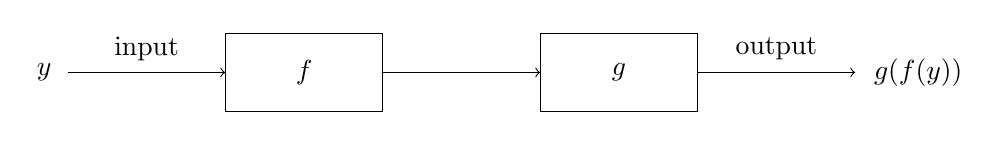
\begin{tikzpicture}
\draw (0,0.5) rectangle (2,1.5);
\draw (4,0.5) rectangle (6,1.5);

\node at (1,1) {$f$};
\node at (5,1) {$g$};
\node at (-2.3, 1) {$y$};
\node at (8.8, 1) {$g(f(y))$};

\draw[->] (-2,1) -- (0,1);
\draw[->] (2,1) -- (4,1);
\draw[->] (6,1) -- (8, 1); 


\node at (-1, 1.3) {input};
\node at (7, 1.3) {output};
\end{tikzpicture}

\emph{The function $g \circ f$.}
\end{center}